% 5. Section: Training and Evaluation Paradigm
\section{Training and Evaluation Paradigm}
\label{ch:experimental_design}

\subsection{Training Environment and Hyperparameter Configuration}
\label{sec:exp_training_env}
% Specification of the computational setup (PyTorch Lightning, WandB for experiment tracking and logging) and critical hyperparameters. Configuration management via Pydantic. List of hyperparameters (e.g., batch size, learning rate, number of epochs, etc.) and their respective values. Discussion of the rationale behind the selected configurations.
The training and evaluation environment uses a robust and reproducible setup. The entire suite for training, evaluation, and logging is managed through PyTorch Lightning, with experiment tracking and visualization handled by Weights \& Biases (WandB). This setup allows for managed logging, checkpointing, and distributed training strategies. Pydantic manages all configuration and hyperparameters, which enables a ``Config-as-Factory'' pattern that makes it easy to swap different models, datasets, or loss functions. The data loading pipeline uses HDF5 for high throughput. For efficient processing, the framework randomly partitions the full sample index into 32 shards and assigns one shard to each DataLoader worker to ensure balanced and parallel prefetching. The provided documentation does not detail specific hyperparameters such as batch size and learning rate.
 
\subsection{Optimization Strategy and Learning Objective}
\label{sec:exp_optimization}
\subsubsubsection{Loss Function Formulation}
% Detailed specification of the loss function(s) employed for MTR training, including components for trajectory regression and mode probability classification. Discussion of how this objective function guides the model to learn multimodal distributions (e.g., relationship to Brier-FDE if incorporated).
The UniTraj framework unifies loss functions for different models. The overall training objective is to minimize these functions to improve prediction accuracy. The training process specifically seeks to decrease metrics such as the minimum Final Displacement Error (FDE), as illustrated by the training graphs. A key component of the learning objective is the Brier Final Displacement Error, which evaluates both the accuracy of the trajectory's final point and the model's confidence in that prediction. Figure \ref{fig:mtr_prediction} shows an example of a multimodal prediction, where the model outputs several possible future paths with associated probabilities. The exact mathematical formulation of the loss function used for the Motion Transformer (MTR) training run is not specified in the source material.
 
% toDO(luroess): Generate new visualization for MTR prediction, this looks awful
\begin{figure}[htbp]
    \centering
    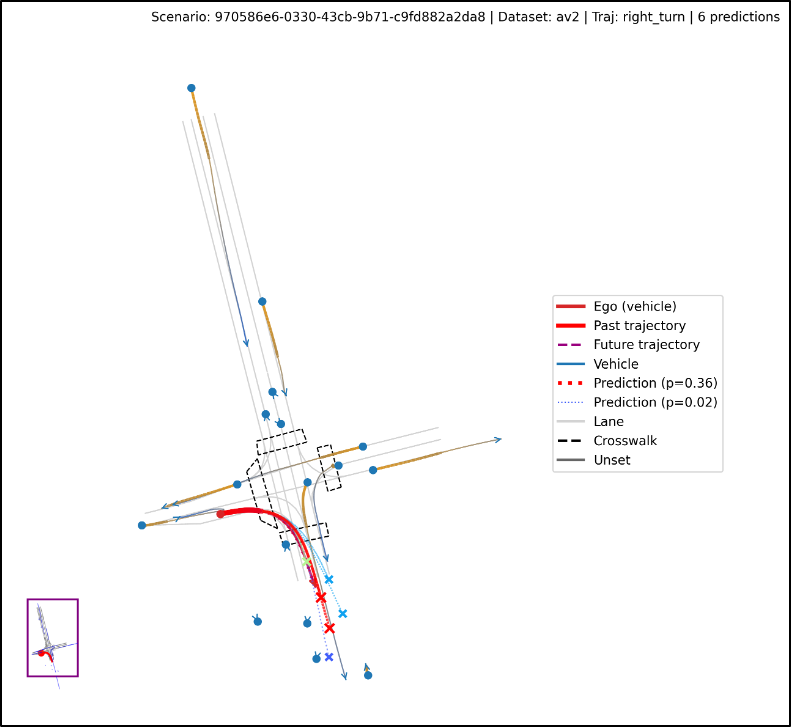
\includegraphics[width=0.8\textwidth]{figures/input_output_viz_ugly.png}
    \caption{A multimodal prediction from the MTR model for a right-turn scenario. The model generates multiple future trajectories, assigning a probability to each. The green line is the ground truth future path, while the colored lines are predictions, with one having a much higher probability (p=0.36) than another (p=0.02).}
    \label{fig:mtr_prediction}
\end{figure}
 
\subsubsubsection{Optimizer Selection}
% e.g., Adam optimizer with specified learning rate and scheduling.
The specific optimization algorithm, such as Adam or SGD, and its associated parameters like learning rate and scheduling, are not mentioned in the provided documentation.
 
\subsection{Evaluation Metrics}
\label{sec:exp_metrics}
The performance of the trajectory prediction model is assessed using a set of standard industry metrics. The mathematical definitions for these metrics are as follows:
\begin{itemize}
 \item \textbf{Average Displacement Error (ADE):} The mean L2 distance between the predicted trajectory and the ground truth over all time steps, defined as $ADE=\mathbb{E}_{t}[||\hat{y}_{t}-y_{t}||_{2}]$.
 \item \textbf{Final Displacement Error (FDE):} The L2 distance between the predicted final position and the ground truth final position, defined as $FDE=||\hat{y}_{T}-y_{T}||_{2}$.
 \item \textbf{Miss Rate (MR):} The fraction of predictions where the final displacement error for the best trajectory candidate exceeds a distance threshold $d_{thresh}$ (e.g., 2.0 m). The formula is $MR=\mathbb{E}_{k}[\mathbb{I}\{||\hat{y}_{T}^{(k)}-y_{T}||_{2}>d_{thresh}\}]$.
 \item \textbf{Brier Final Displacement Error (BrierFDE):} A metric that scores both the trajectory accuracy and the probability assigned to it, defined as $BrierFDE=\mathbb{E}_{k}[p_{k}\cdot||\hat{y}_{T}^{(k)}-y_{T}||_{2}^{2}]$.
\end{itemize}
On the validation set, the trained MTR model achieved a \textbf{brier-minFDE} of 1.98, a \textbf{minFDE} of 1.6655, a \textbf{minADE} of 0.86294, and a \textbf{Miss Rate} of 0.30141. These results are comparable to baseline values from existing literature. The Brier-FDE of 1.98 shows a slight improvement over the 2.08 value reported in the MTR paper's appendix. Figure \ref{fig:validation_metrics} shows the progression of these metrics on the validation set over the course of training.

% toDO(luroess): Split graphs for better vizualization?
\begin{figure}[htbp]
    \centering
    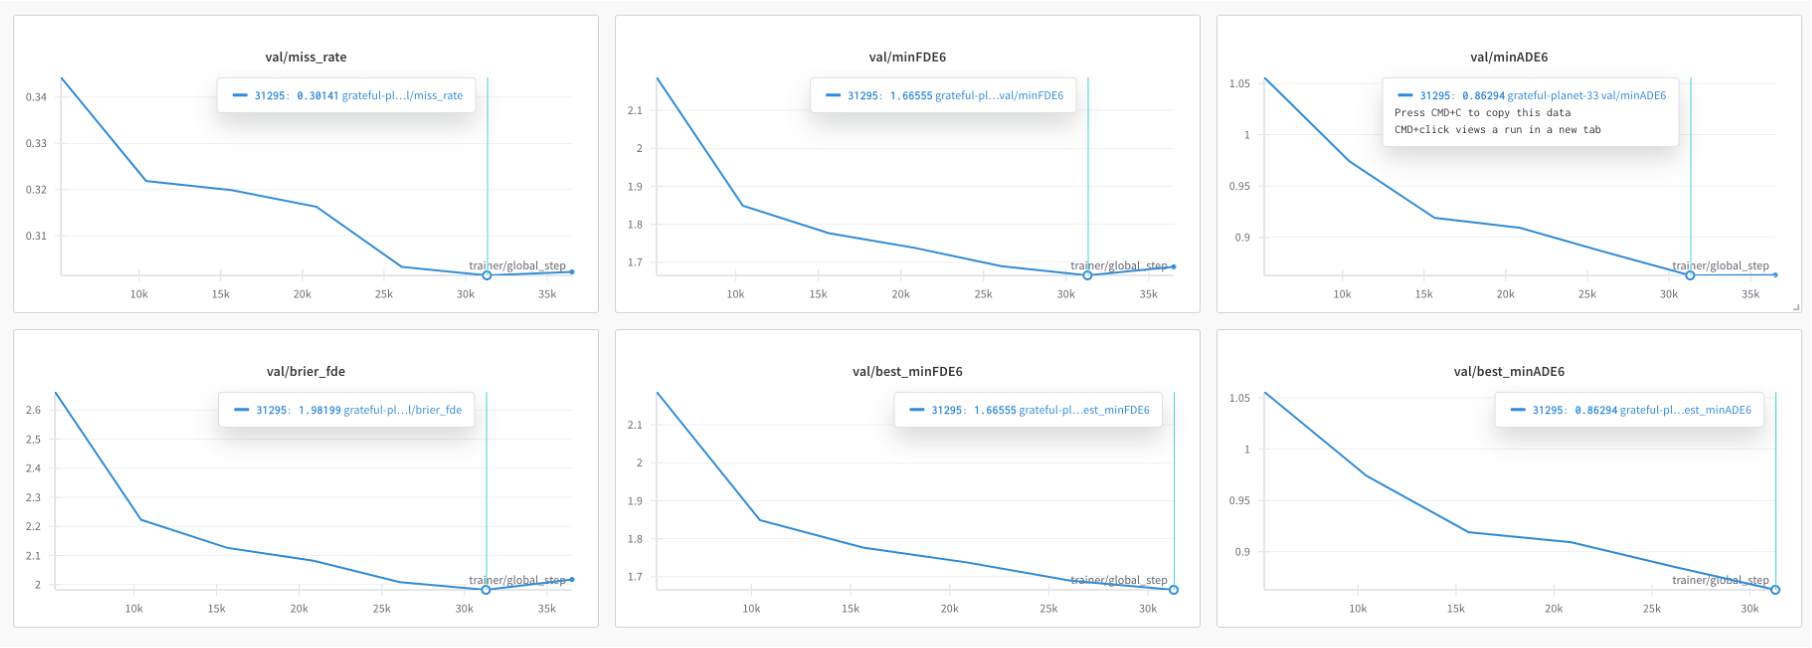
\includegraphics[width=\textwidth]{figures/performance_metrics_validation.png}
    \caption{Performance metrics on the validation set during MTR training. The plots show a consistent decrease in error for miss rate, FDE, ADE, and Brier-FDE as training progresses. The final reported values are taken at step 31,295.}
    \label{fig:validation_metrics}
\end{figure}

\subsection{Training Paradigm}
\label{sec:model_training_paradigm}
\subsubsubsection{Learning Objective and Loss Function(s)}
\label{sec:model_loss_functions}
   % - The overall objective the model is trained to optimize.
   % - Specific loss components and their roles.
   % - e.g., For MTR: Gaussian Regression Loss (NLL) and auxiliary L1 regression loss. 
   % - Any specific strategies like hard assignment in MTR. 
The primary learning objective is to train the model to accurately forecast multimodal trajectories. The training process, tracked over thousands of steps, shows a clear reduction in loss values for metrics including minFDE6, minADE6, and miss rate, indicating the model is learning from the data. Figure \ref{fig:training_metrics_grid} illustrates this by charting the decrease across multiple training metrics. The framework's design principle is to unify loss functions across different models, and the training objective is to minimize the selected loss function to achieve better performance on the evaluation metrics.

% toDO(luroess): Split graphs for better vizualization?
\begin{figure}[htbp]
    \centering
    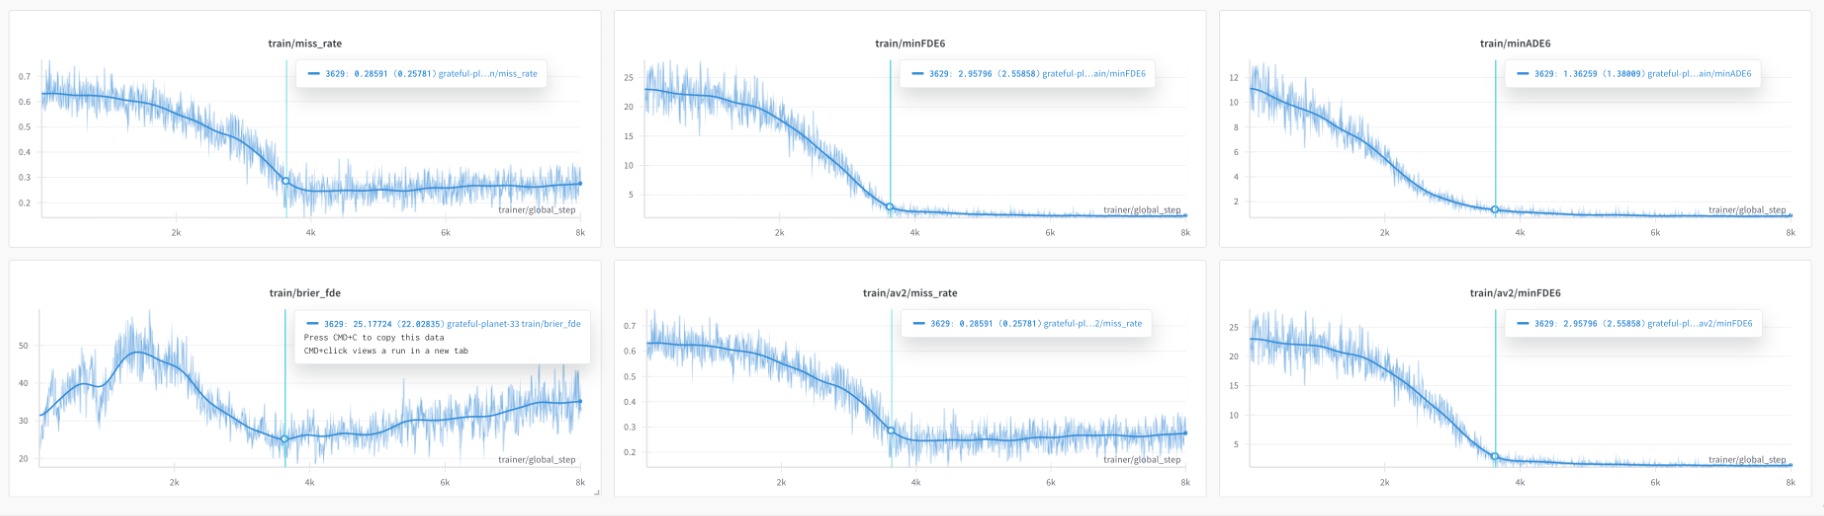
\includegraphics[width=\textwidth]{figures/performance_metrics_training.png}
    \caption{A grid of performance metrics on the training set. The plots show a consistent decrease in error for miss rate, brier FDE, minFDE6, and minADE6 over approximately 6,000 training steps, which indicates successful learning.}
    \label{fig:training_metrics_grid}
\end{figure}

\subsubsubsection{Optimization Strategy and Training Details}
\label{sec:model_optimization_details}
   % - Optimizer used, learning rate, batch size, epochs etc. 
   % - How iterative improvements are achieved during training (e.g. loss on intermediate decoder layers for MTR ).
The MTR model was trained from scratch without using a pre-trained model. A significant part of the setup involved adapting the model to the UniTraj framework's data parsing and configuration systems. The training data undergoes a detailed processing pipeline. First, the pipeline selects agents from scenarios based on type (vehicle, pedestrian, or cyclist), movement distance, and visibility. Scenarios are also categorized by difficulty (Easy, Medium, Hard) based on a Kalman filter analysis. Subsequently, the system normalizes all coordinate data into an agent-centric frame using the rotation matrix $R_{z}(-\theta_{c})$. Finally, it assembles agent and map features into padded and masked tensors of dimensions $\mathbb{R}^{N_{max}\times T_{p}\times F_{ap}}$ for dynamic data and $\mathbb{R}^{K\times L\times F_{map}}$ for static map data, preparing them for model ingestion.
